%\newpage

\section{Performance data and analysis}
\label{performance}

We measured the EPCC benchmark using various barrier designs to show
the differences in performance overhead. 


Figure \ref{fig:power4performance} shows the barrier overhead for each
kind of implementations on a 32-way POWER4 system with varying numbers
of threads. We used different labels to tag different designs.
\emph{FetchAndAdd} is for the first and the simplest barrier design.
\emph{DistCounter} is used for the barrier with distributed counter.
\emph{DistCounterPad} is used for the barrier with padded distributed
counter. \emph{LocalSensor} is for the barrier using local sensor. And
the last one, \emph{Combined} represents our new barrier scheme, the
barrier with distributed counter combined with local sensor.

\begin{figure*}[!htbp]
  \begin{center}
    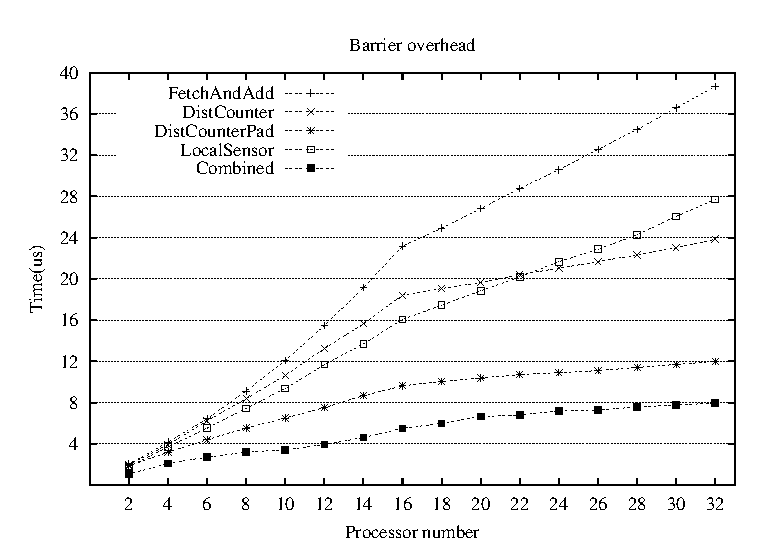
\includegraphics[angle=0, width=0.9\textwidth]{power4performance.eps}
    \caption{POWER4 barrier overhead}
    \label{fig:power4performance}
  \end{center}
\end{figure*}

To further understand the behavior of these barrier designs, we
repeated the tests on a 16-way 375MHz POWER3 system.  Figure
\ref{fig:power3performance} shows the overheads on POWER3.

\begin{figure*}[!htbp]
  \begin{center}
    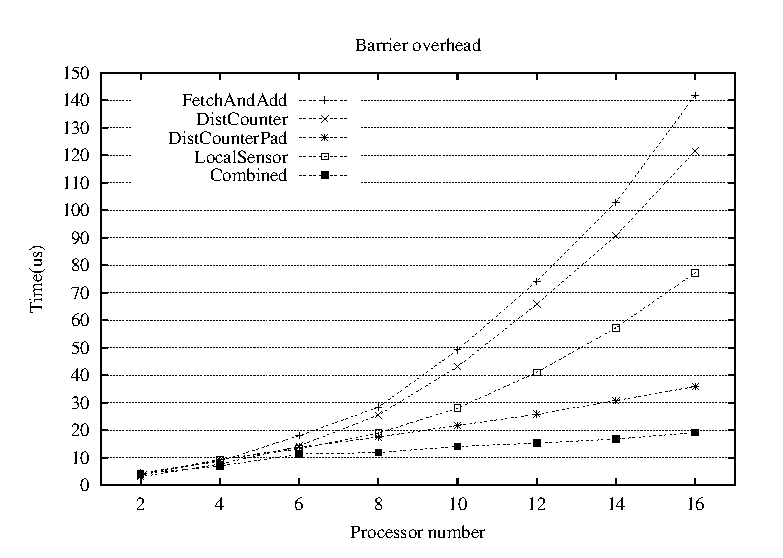
\includegraphics[angle=0, width=0.9\textwidth]{power3performance.eps}
    \caption{POWER3 barrier overhead}
    \label{fig:power3performance}
  \end{center}
\end{figure*}

Although POWER4 and POWER3 have different memory
architectures\cite{Ste98}, one can see that there is little difference
in the relative overhead for different barrier designs. Of course, we
could not compare the scalability of the designs beyond 16 threads on
the POWER3 system so a completely equitable comparison was not
possible.

From the figures we can see that the scalability of the overhead
is not exactly the same, even considering the difference of the clock
speed of the processors --- recall that the POWER4 system we used is
1.1GHz and the POWER3 is 375MHz. The memory system in POWER4 system
certainly gives it extra advantage.

To be able to compare the different implementations, we examine the
performance counters on the more interesting POWER4 system, using
\texttt{pmcount} program available on AIX 5.1. The program will print
out the values of the different performance counters on each
processor, when monitoring a given execution program.

\begin{figure*}[!h]
  \begin{center}
    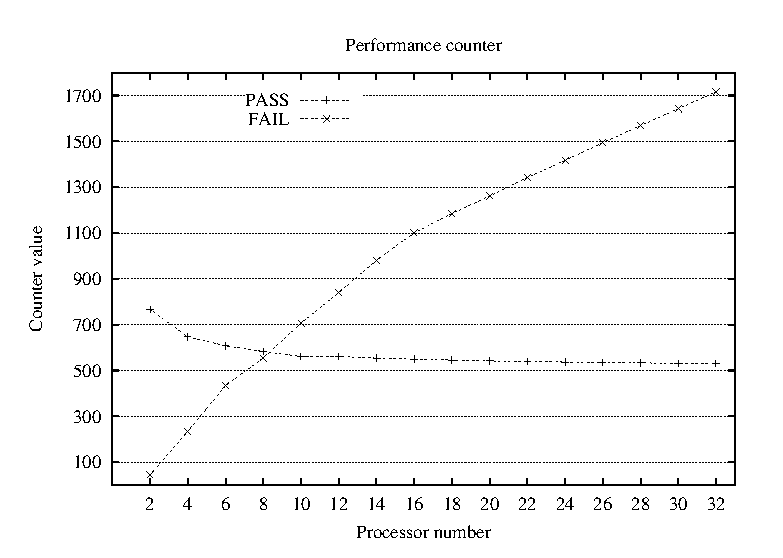
\includegraphics[angle=0, width=0.9\textwidth]{stcx.eps}
    \caption{Store conditional instruction pass and fail}
    \label{fig:stcx}
    \end{center}
\end{figure*}

First we do a simple measurement for the fetch-and-add barrier, using
the exact same setting as we measure overhead previously. We check the
performance counter for store conditional instruction to see the
relationship between contention and the number of processors involved
in a barrier operation. Figure \ref{fig:stcx} shows the average number
of pass and fail for the store conditional instructions on each
processor.

As one can see, while the number of pass remained almost the same(in
theory, it should be identical since we have the same number of
barrier for different number of processors, we consider it is
measurement error here), the number of fail increased sharply as more
processors are added.  That explains why we can not have a scalable
performance for fetch-and-add barrier.

%The barrier implemented with local sensor will has the same problem.

Similarly, we can get the performance counter for cache misses,
representing data traffic. An interesting case here is L2 miss for
distributed counter.

For a POWER4 system, an L2 miss may be served by L2 from another L2 in
the same MCM, L2 in a different MCM, L3 in the same MCM and L3 in a
different MCM. We put them all together as L2 misses. Figure
\ref{fig:lsource} pictures average L2 misses on different processors
for barrier with distributed counter and padded distributed counter.

\begin{figure*}[!h]
  \begin{center}
    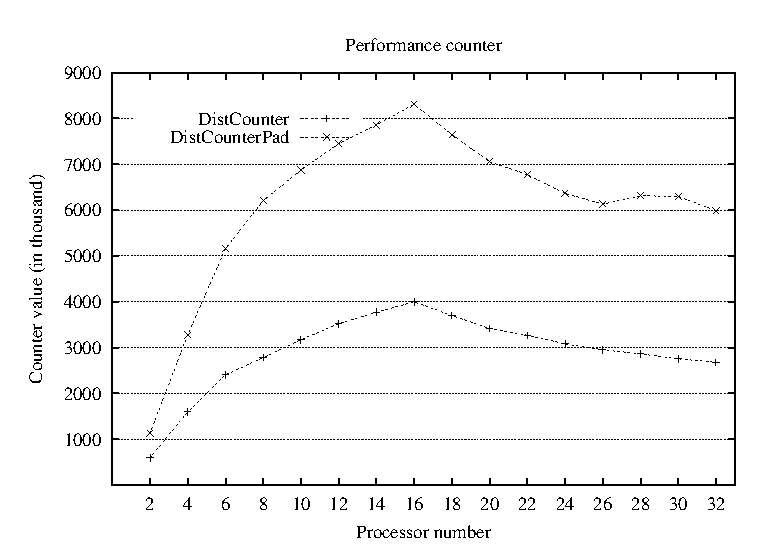
\includegraphics[angle=0, width=0.9\textwidth]{lsource.eps}
    \caption{L2 misses}
    \label{fig:lsource}
    \end{center}
\end{figure*}

To our surprise, there are more cache misses in the barrier with
padded counter, even though it cost less time. We are not sure what
exactly caused this, but we suspect that the cache coherent algorithm
used in hardware cause extra contention when different processors
accessing the same cache line, which out weighs the traffic overhead
caused by L2 misses.

%\begin{verbatim}
%...
%[We are currently working to measure performance 
%counters and analyzing the data.
%The results will be added in the final version of the paper.]
%\end{verbatim}

%Figure \ref{fig:l2misses} shows the mean number of L2 cache misses
%that occurred in all the caches during the execution of 500,000
%barriers as a function of the number of threads participating in the
%barrier. Similarly, Figure \ref{fig:l3misses} shows the L3 cache
%miss behavior (main memory accesses).  Note that, unlike in Figure \ref{fig:l2misses}, the units are not in thousands.

%\begin{figure*}[!htbp]
%  \begin{center}
%    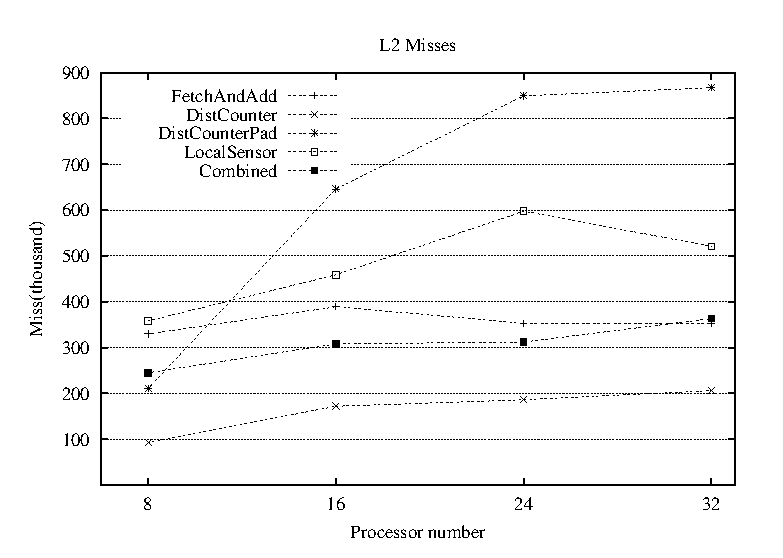
\includegraphics[angle=0, width=0.95\textwidth]{l2miss.eps}
%    \caption{L2 cache misses}
%    \label{fig:l2misses}
%    \end{center}
%\end{figure*}

%\begin{figure*}[!htbp]
%  \begin{center}
%    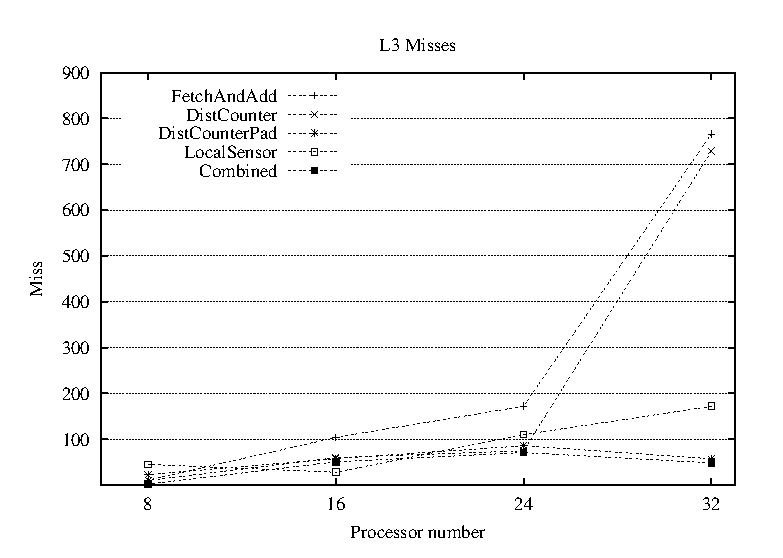
\includegraphics[angle=0, width=0.95\textwidth]{l3miss.eps}
%    \caption{L3 cache misses}
%    \label{fig:l3misses}
%    \end{center}
%\end{figure*}

%We see that the fetch-and-add implementation suffers from a large
%contention problem.  All threads are accessing the same memory location
%at the same time, either signaling arrival or checking if the
%barrier counter is zero. This explains the relatively high number of cache
%misses (including both second and third level) compared to the other
%implementations.

%Each time a given thread reaches the barrier, it has to update the
%counter (and compete for the counter via the fetch-and-add atomic
%operation) and then spin on that counter looking for all changes. This
%will generate a considerable amount of memory traffic as threads will try
%to access the memory position but will need to obtain a valid copy due to
%intervening writes. One
%by one, threads will grab the counter and invalidate all cache lines
%of the other spinning processors.  This will induce all other
%processors to issue a new request for data, forcing a new miss in the cache.
%When the $n^{th}$ thread updates the counter, all spinning threads
%will have their cache line invalidated and will request the line again,
%causing $(n-1)$ misses (1 per cache).

%In total, the first thread that reaches the barrier will fail $(n-1)$
%times due to this effect while the last one will not have misses (but
%will have misses for accessing the counter). This justifies why it has
%the worst L3 behavior, and why it does not scale smoothly.

%The second implementation, DistCounter, mitigates this cache coherence problem to some
%degree. Threads spin in different memory positions (avoiding
%contention) even though the distributed counters share a cache line with some
%other distributed counters.  This barrier implementation also saves overhead
%by avoiding the need for an atomic memory operation.

%We can see that this behavior is greatly reflected in the
%number of L2 cache misses.  The scalability curve has changed from a rather steep line to a
%flatter one. This is mainly due to the fact that the weight of the
%barrier is in the first phase of signaling arrival. The first
%implementation uses fetch-and-add, while the second uses a simple
%store. Nevertheless, false sharing is
%encountered due to the sharing of cache lines among counters.  This explains the L3 cache behavior.

%In contrast, the third implementation, DistCounterPad, is similar to
%DistCounter but tries to eliminate the false sharing problem. Placing
%the whole distributed counter into only one cache line has the
%inconvenience that only one processor can have that line in modified
%state.  The padding tries to enhance the behavior by reducing the
%number of external invalidations.  However, it has a bad L2 cache
%behavior, but as L3 is more important for the overall execution time,
%it is faster than the previous one.

%Each of these techniques addresses the ``entry'' phase of the barrier.  We will see now the effect of optimizing the ``exit'' phase.

%The LocalSensor implementation, which uses a fetch-and-add mechanism,
%is the first one to reduce the overhead in the ``exit'' phase of a
%barrier. Since it does nothing to improve the ``entry'' phase, we get
%better behavior than the first barrier, but not significantly better
%from the DistCounter and DistCounterPad implementations.

%Not surprisingly, the Combined implementation, that benefits from an
%enhanced behavior in both phases, performs better than all the other
%implementations. This is due to the fact that the number of L3 misses
%decreases significantly because of the low degree of communication. Each
%cache line will be accessed only by its corresponding thread and one additional time by the master
%thread.  These cache lines will have no other remote accesses, regardless of
%the number of threads participating in the barrier. That gives us a rather flat line,
%and explains why this implementation is considerably more scalable
%than the previously studied barrier designs.

